In this chapter, we provide the context that forms the basis of our research. We begin by presenting a broad overview of the study of brain function, before narrowing down to the specific field of task-based Blood-Oxygen-Level-Dependent (BOLD) functional Magnetic Resonance Imaging (MRI) that will be the main focus of study in this thesis. Here, we describe each of the preprocessing and modelling components of a typical task-fMRI analysis pipeline. Finally, we give an in-depth discussion of the state-of-the-art procedures used for subject- and group-level fMRI inference that are of particular relevance to the remaining chapters of this work. 

\pagebreak

\section{The Study of Brain Function}

\begin{figure}[htbp]
\centering
	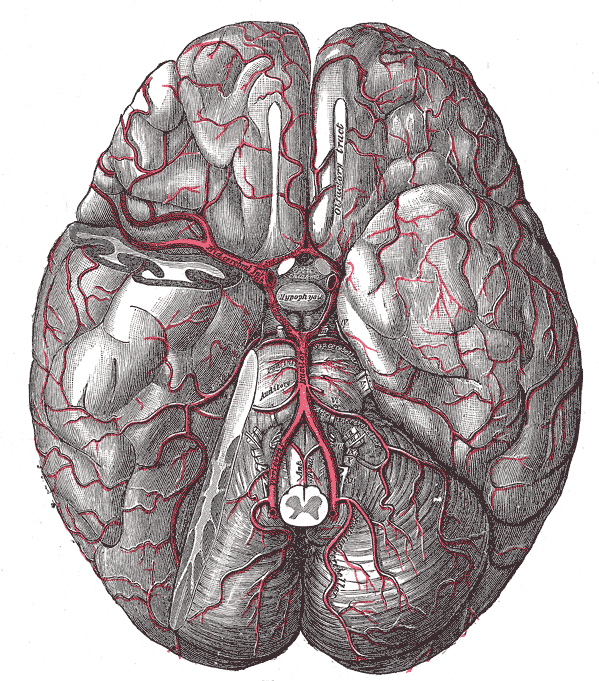
\includegraphics[height=3in]{1_Grays_Anatomy.png}	
\caption*{\textbf{Figure 1:} An illustration showing the arteries at the base of the human brain from (Gray, 1918).}
\end{figure}

The human brain, the central organ of the human nervous system, has been described as one of the most complex structures in the known universe. Made up of approximately 86 billion neurons (Azevedo et al., 2009), where neuronal interaction occurs continuously via trillions of synaptic networks to form intricate and dynamic neural networks, the myriad of processes taking place inside the brain at any given time make the study of brain function an intimidating challenge. Nonetheless, our understanding of this organ has come along way from our ancient Egyptian ancestors, who believed that the heart was at the source of human intelligence, and for whom the practice of drilling a hole into the skull was regarded as a solution to cure a headache. 

Remarkably, much of this progress has come in the last century alone. A number of key developments within this time-frame include: Confirmation of the neuron doctrine, the concept that the nervous system is a collection of discrete individual cells, postulated by Santiago Ramon y Cajal at the end of the 19th century and demonstrated in the 1950s thanks to the development of electron microscopy; the first evidence of neuroplasticity, the ability for the brain's structure to change during an individual's lifetime; and the emergence of neuroimaging techniques such as electroencephalography (EEG), positron emisson tomography (PET), and MRI.    

\section{Magnetic Resonance Imagery (MRI)}

\section{Task-based functional Magnetic Resonance Imagery (t-fMRI)}

\subsection{Overview}

\subsection{Pre-processing}

\section{Statistical Analysis: Subject-level}

\subsection{Parametric Methods}

\subsection{Nonparametric Methods}

\section{Statistical Analysis: Group-level}

\subsection{Parametric Methods}

\subsection{Nonparametric Methods}

\section{Reproducibility of fMRI Results}

